% 2025_shanghai_spring_q13_fig1: 正四棱台 ABCD-A1B1C1D1 示意（schematic 投影）
\usetikzlibrary{calc}
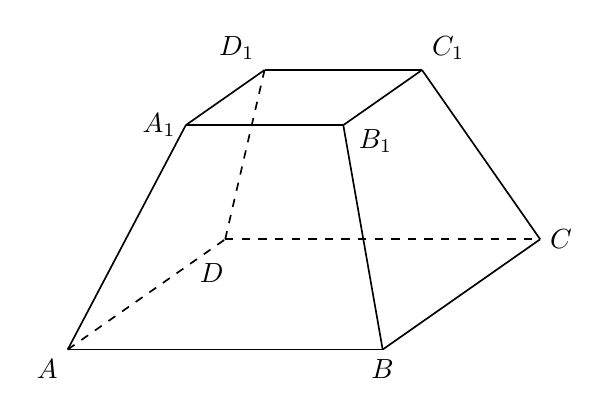
\begin{tikzpicture}[x=1cm,y=1cm,line width=.6pt]
  % 底部（大）与顶部（小）投影坐标
  \coordinate (A) at (0.0000000000,0.0000000000);
  \coordinate (B) at (4.0000000000,0.0000000000);
  \coordinate (C) at (6.0000000000,1.4000000000);
  \coordinate (D) at (2.0000000000,1.4000000000);
  \coordinate (A1) at (1.5000000000,2.8500000000);
  \coordinate (B1) at (3.5000000000,2.8500000000);
  \coordinate (C1) at (4.5000000000,3.5500000000);
  \coordinate (D1) at (2.5000000000,3.5500000000);
  % 可见底边与侧棱
  \draw (A) -- (B);
  \draw (B) -- (C);
  \draw (A) -- (A1);
  \draw (B) -- (B1);
  \draw (C) -- (C1);
  % 顶面四边（可见）
  \draw (A1) -- (B1);
  \draw (B1) -- (C1);
  \draw (C1) -- (D1);
  \draw (D1) -- (A1);
  % 遮挡边（虚线）
  \draw[dashed] (A) -- (D);
  \draw[dashed] (D) -- (C);
  \draw[dashed] (D) -- (D1);
  % D 处直角标记（原图 D 附近小折线，示意顶面/侧面垂直关系）
    % 标签（紧邻对应点，避碰）
  \node[below left,font=\normalsize] at (A) {$A$};
  \node[below,font=\normalsize] at (B) {$B$};
  \node[right,font=\normalsize] at (C) {$C$};
  \node[below left,font=\normalsize,xshift=3pt,yshift=-5pt] at (D) {$D$};
  \node[left,font=\normalsize] at (A1) {$A_1$};
  \node[below right,font=\normalsize,xshift=2.0pt,yshift=2pt] at (B1) {$B_1$};
  \node[above right,font=\normalsize] at (C1) {$C_1$};
  \node[above left,font=\normalsize] at (D1) {$D_1$};
\end{tikzpicture}
